% fig_gac_framework.tex — GAC Framework Pipeline
% Usage: % fig_gac_framework.tex — GAC Framework Pipeline
% Usage: % fig_gac_framework.tex — GAC Framework Pipeline
% Usage: % fig_gac_framework.tex — GAC Framework Pipeline
% Usage: \input{figures/fig_gac_framework.tex}
\begin{figure*}[t]
\centering
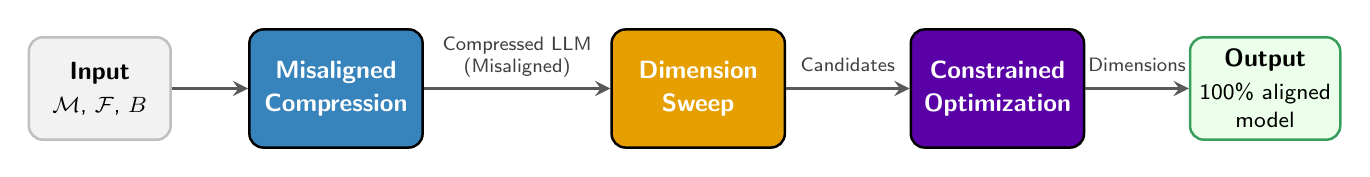
\begin{tikzpicture}[scale=1.0, every node/.style={scale=1.0},
    >=stealth,
    % Colors
    cblue/.style={fill={rgb,255:red,55;green,131;blue,187}},
    cred/.style={fill={rgb,255:red,211;green,63;blue,73}},
    cgreen/.style={fill={rgb,255:red,56;green,158;blue,92}},
    corange/.style={fill={rgb,255:red,230;green,159;blue,0}},
    % Styles
    phase/.style={draw, rounded corners=5pt, minimum width=2.2cm, minimum height=1.5cm,
                  line width=0.9pt, font=\sffamily\small, align=center},
    iobox/.style={draw, rounded corners=5pt, minimum width=1.8cm, minimum height=1.3cm,
                  line width=0.9pt, font=\sffamily\small, align=center},
    arrow/.style={->, line width=1.4pt, color=gray!70!black},
    lbl/.style={font=\sffamily\scriptsize, align=center, text=gray!50!black},
  ]

  % Input
  \node[iobox, fill=gray!10, draw=gray!50] (input) at (0, 0) {
    \textbf{Input}\\[1pt]
    {\footnotesize $\mathcal{M}$, $\mathcal{F}$, $B$}
  };

  % Step 1: Unconstrained Compression
  \node[phase, cblue, text=white] (compress) at (3.0, 0) {
    \textbf{Misaligned}\\[1pt]
    \textbf{Compression}
  };

  % Step 2: Dimension Sweep
  \node[phase, corange, text=white] (sweep) at (7.6, 0) {
    \textbf{Dimension}\\[1pt]
    \textbf{Sweep}
  };

  % Step 3: Knapsack DP
  \node[phase, fill=violet!70!blue, text=white] (dp) at (11.4, 0) {
    \textbf{Constrained}\\[1pt]
    \textbf{Optimization}
  };

  % Output
  \node[iobox, fill=green!8, draw={rgb,255:red,56;green,158;blue,92}] (output) at (14.8, 0) {
    \textbf{Output}\\[1pt]
    {\footnotesize 100\% aligned}\\[-1pt]
    {\footnotesize model}
  };

  % Arrows
  \draw[arrow] (input) -- (compress);
  \draw[arrow] (compress) -- (sweep) node[midway, above=0pt, lbl] {Compressed LLM\\(Misaligned)};
  \draw[arrow] (sweep) -- (dp) node[midway, above=2pt, lbl] {Candidates};
  \draw[arrow] (dp) -- (output) node[midway, above=2pt, lbl] {Dimensions};

\end{tikzpicture}
\caption{GAC Pipeline.}
\label{fig:gac_framework}
\end{figure*}

\begin{figure*}[t]
\centering
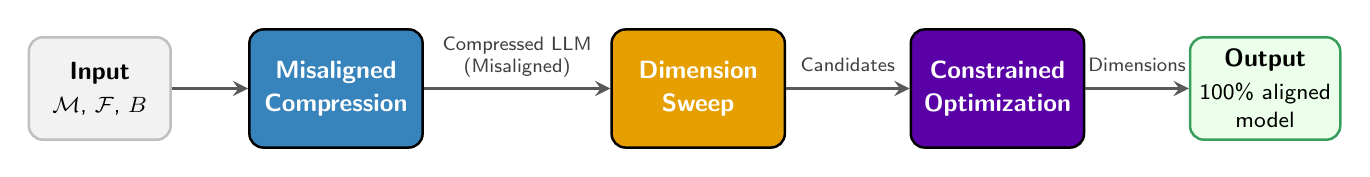
\begin{tikzpicture}[scale=1.0, every node/.style={scale=1.0},
    >=stealth,
    % Colors
    cblue/.style={fill={rgb,255:red,55;green,131;blue,187}},
    cred/.style={fill={rgb,255:red,211;green,63;blue,73}},
    cgreen/.style={fill={rgb,255:red,56;green,158;blue,92}},
    corange/.style={fill={rgb,255:red,230;green,159;blue,0}},
    % Styles
    phase/.style={draw, rounded corners=5pt, minimum width=2.2cm, minimum height=1.5cm,
                  line width=0.9pt, font=\sffamily\small, align=center},
    iobox/.style={draw, rounded corners=5pt, minimum width=1.8cm, minimum height=1.3cm,
                  line width=0.9pt, font=\sffamily\small, align=center},
    arrow/.style={->, line width=1.4pt, color=gray!70!black},
    lbl/.style={font=\sffamily\scriptsize, align=center, text=gray!50!black},
  ]

  % Input
  \node[iobox, fill=gray!10, draw=gray!50] (input) at (0, 0) {
    \textbf{Input}\\[1pt]
    {\footnotesize $\mathcal{M}$, $\mathcal{F}$, $B$}
  };

  % Step 1: Unconstrained Compression
  \node[phase, cblue, text=white] (compress) at (3.0, 0) {
    \textbf{Misaligned}\\[1pt]
    \textbf{Compression}
  };

  % Step 2: Dimension Sweep
  \node[phase, corange, text=white] (sweep) at (7.6, 0) {
    \textbf{Dimension}\\[1pt]
    \textbf{Sweep}
  };

  % Step 3: Knapsack DP
  \node[phase, fill=violet!70!blue, text=white] (dp) at (11.4, 0) {
    \textbf{Constrained}\\[1pt]
    \textbf{Optimization}
  };

  % Output
  \node[iobox, fill=green!8, draw={rgb,255:red,56;green,158;blue,92}] (output) at (14.8, 0) {
    \textbf{Output}\\[1pt]
    {\footnotesize 100\% aligned}\\[-1pt]
    {\footnotesize model}
  };

  % Arrows
  \draw[arrow] (input) -- (compress);
  \draw[arrow] (compress) -- (sweep) node[midway, above=0pt, lbl] {Compressed LLM\\(Misaligned)};
  \draw[arrow] (sweep) -- (dp) node[midway, above=2pt, lbl] {Candidates};
  \draw[arrow] (dp) -- (output) node[midway, above=2pt, lbl] {Dimensions};

\end{tikzpicture}
\caption{GAC Pipeline.}
\label{fig:gac_framework}
\end{figure*}

\begin{figure*}[t]
\centering
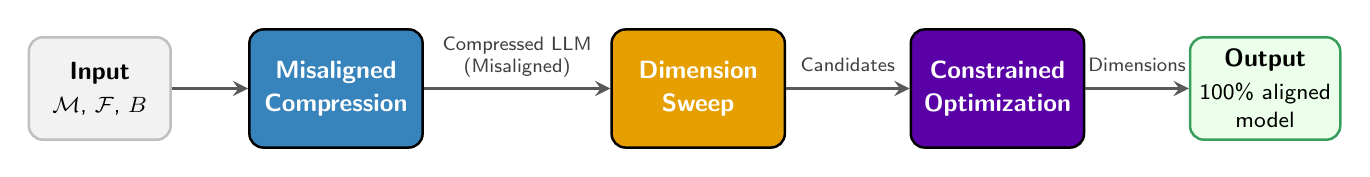
\begin{tikzpicture}[scale=1.0, every node/.style={scale=1.0},
    >=stealth,
    % Colors
    cblue/.style={fill={rgb,255:red,55;green,131;blue,187}},
    cred/.style={fill={rgb,255:red,211;green,63;blue,73}},
    cgreen/.style={fill={rgb,255:red,56;green,158;blue,92}},
    corange/.style={fill={rgb,255:red,230;green,159;blue,0}},
    % Styles
    phase/.style={draw, rounded corners=5pt, minimum width=2.2cm, minimum height=1.5cm,
                  line width=0.9pt, font=\sffamily\small, align=center},
    iobox/.style={draw, rounded corners=5pt, minimum width=1.8cm, minimum height=1.3cm,
                  line width=0.9pt, font=\sffamily\small, align=center},
    arrow/.style={->, line width=1.4pt, color=gray!70!black},
    lbl/.style={font=\sffamily\scriptsize, align=center, text=gray!50!black},
  ]

  % Input
  \node[iobox, fill=gray!10, draw=gray!50] (input) at (0, 0) {
    \textbf{Input}\\[1pt]
    {\footnotesize $\mathcal{M}$, $\mathcal{F}$, $B$}
  };

  % Step 1: Unconstrained Compression
  \node[phase, cblue, text=white] (compress) at (3.0, 0) {
    \textbf{Misaligned}\\[1pt]
    \textbf{Compression}
  };

  % Step 2: Dimension Sweep
  \node[phase, corange, text=white] (sweep) at (7.6, 0) {
    \textbf{Dimension}\\[1pt]
    \textbf{Sweep}
  };

  % Step 3: Knapsack DP
  \node[phase, fill=violet!70!blue, text=white] (dp) at (11.4, 0) {
    \textbf{Constrained}\\[1pt]
    \textbf{Optimization}
  };

  % Output
  \node[iobox, fill=green!8, draw={rgb,255:red,56;green,158;blue,92}] (output) at (14.8, 0) {
    \textbf{Output}\\[1pt]
    {\footnotesize 100\% aligned}\\[-1pt]
    {\footnotesize model}
  };

  % Arrows
  \draw[arrow] (input) -- (compress);
  \draw[arrow] (compress) -- (sweep) node[midway, above=0pt, lbl] {Compressed LLM\\(Misaligned)};
  \draw[arrow] (sweep) -- (dp) node[midway, above=2pt, lbl] {Candidates};
  \draw[arrow] (dp) -- (output) node[midway, above=2pt, lbl] {Dimensions};

\end{tikzpicture}
\caption{GAC Pipeline.}
\label{fig:gac_framework}
\end{figure*}

\begin{figure*}[t]
\centering
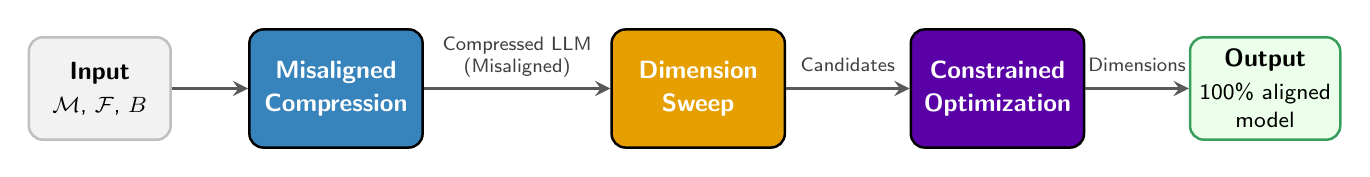
\begin{tikzpicture}[scale=1.0, every node/.style={scale=1.0},
    >=stealth,
    % Colors
    cblue/.style={fill={rgb,255:red,55;green,131;blue,187}},
    cred/.style={fill={rgb,255:red,211;green,63;blue,73}},
    cgreen/.style={fill={rgb,255:red,56;green,158;blue,92}},
    corange/.style={fill={rgb,255:red,230;green,159;blue,0}},
    % Styles
    phase/.style={draw, rounded corners=5pt, minimum width=2.2cm, minimum height=1.5cm,
                  line width=0.9pt, font=\sffamily\small, align=center},
    iobox/.style={draw, rounded corners=5pt, minimum width=1.8cm, minimum height=1.3cm,
                  line width=0.9pt, font=\sffamily\small, align=center},
    arrow/.style={->, line width=1.4pt, color=gray!70!black},
    lbl/.style={font=\sffamily\scriptsize, align=center, text=gray!50!black},
  ]

  % Input
  \node[iobox, fill=gray!10, draw=gray!50] (input) at (0, 0) {
    \textbf{Input}\\[1pt]
    {\footnotesize $\mathcal{M}$, $\mathcal{F}$, $B$}
  };

  % Step 1: Unconstrained Compression
  \node[phase, cblue, text=white] (compress) at (3.0, 0) {
    \textbf{Misaligned}\\[1pt]
    \textbf{Compression}
  };

  % Step 2: Dimension Sweep
  \node[phase, corange, text=white] (sweep) at (7.6, 0) {
    \textbf{Dimension}\\[1pt]
    \textbf{Sweep}
  };

  % Step 3: Knapsack DP
  \node[phase, fill=violet!70!blue, text=white] (dp) at (11.4, 0) {
    \textbf{Constrained}\\[1pt]
    \textbf{Optimization}
  };

  % Output
  \node[iobox, fill=green!8, draw={rgb,255:red,56;green,158;blue,92}] (output) at (14.8, 0) {
    \textbf{Output}\\[1pt]
    {\footnotesize 100\% aligned}\\[-1pt]
    {\footnotesize model}
  };

  % Arrows
  \draw[arrow] (input) -- (compress);
  \draw[arrow] (compress) -- (sweep) node[midway, above=0pt, lbl] {Compressed LLM\\(Misaligned)};
  \draw[arrow] (sweep) -- (dp) node[midway, above=2pt, lbl] {Candidates};
  \draw[arrow] (dp) -- (output) node[midway, above=2pt, lbl] {Dimensions};

\end{tikzpicture}
\caption{GAC Pipeline.}
\label{fig:gac_framework}
\end{figure*}
